\chapter{Arquitectura del sistema}
\label{cap:arquitectura}

% TODO: Diagrama general de arquitectura

\section{Visión general}
% TODO

\section{Patrones de diseño}\label{sec:patrones}
\subsection{Microservicios}\label{sec:microservicios}

La plataforma de ``Smart City'' implementada para el Ayuntamiento de San Lorenzo de el Escorial se basa en un diseño orientado a microservicios, es decir, pequeños procesos dedicados a realizar una tarea específica de manera eficiente.

La nueva Web de Turismo del Ayuntamiento se integra también con la plataforma de ``Smart City'' tal y como se puede ver en \ref{sec:webturismo}

Se disponen de distintos tipos de microservicios:

\begin{itemize}
	\item \textbf{Vistas}: Servicios dedicados a gestionar la interconexión con agentes externos (usuarios, vecinos, dispositivos IoT, \ldots)
	\item \textbf{Controladores}: Servicios orientados a resolver tareas específicas
	\item \textbf{Modelos}: Servicios diseñados para interactuar con sistemas de almacenamiento (Bases de datos, \ldots), APIs externas (tiempo metereológico, estado del tráfico, \ldots), o servicios de Inteligencia Artificial (LLMs, TTS, STT, \ldots)
\end{itemize}

\subsubsection{Microservicios de vista}

Estos microservicios son los encargados de interactuar con el mundo exterior a la plataforma de ``Smart City'':

\paragraph{API Gateway}

Este microservicio expone un API REST para las comunicaciones con vecinos, aplicaciones, \ldots

\paragraph{MQTT}

Sistema de colas compatibles con \textbf{MQTT} (utilizando RabbitMQ) para la recepción de eventos de los dispositivos IoT desplegados a lo largo de la ciudad.

\subsection{Comunicación basada en eventos (RPC y Fire-and-Forget)}

De cara a mantener que todos nuestros microservicios sean capades de escalar elásticamente en base a las necesidades de cada momento, se diseñan de manera que cumplan dos casúisticas: `\textit{stateless}' y `\textit{desacoplados}'.

Para poder interconectar todos los microservicios se hace uso de eventos y para su gestión descentralizada se dispone de una plataforma de colas basada en el protocolo \textbf{AMQP} (utilizando RabbitMQ).

Dentro de la pataforma \textbf{AMQP} se disponde de dos tipos de eventos:

\begin{itemize}
	\item RPC: Eventos que esperan una respuesta (\textit{Remote Procedure Call}) y por tanto son síncronos.
	\item Fire\&Forget: Eventos que no esperan una respuesta y por tanto son asíncronos.
\end{itemize}

Todos los microservicios implementados en la plataforma hacen uso de la librería común `Ferimer Queue Manager' (\ref{sec:ferimer-queue-manager}) que 

Esta librería abstrae de la complejidad relativa a la gestión de las comunicaciones de la plataforma \textbf{Atlas}.

\subsection{Ontología de mensajería}

La librería `Atlas Messaging Ontology' (\ref{sec:atlas-messaging-ontology}) define todos los posibles mensajes que se transmiten a través de las colas AMQP de la plataforma así como sus esquemas JSON (\textit{JSON Schemas}) utilizados para validar el correcto formato de las peticiones y sus correspondientes respuestas.

\section{Diagrama de flujo de datos}
% TODO: Diagrama cliente → API → RabbitMQ → servicios

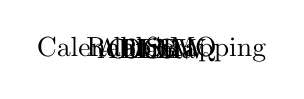
\begin{tikzpicture}[
	]
	\node[] {API GW};
	\node[] {RabbitMQ};
	\node[] {CalendarScrapping};
	\node[] {LLM};
	\node[] {OCR};
	\node[] {Ollama};
\end{tikzpicture}

\section{Seguridad y control de acceso}
% TODO
